\section{Image Segmentation by Active Contour Models in Noisy Images}

Much like in the previous section we start by finding the critical values
of each parameter and seeing how big is its influence in the segmentation.
Then we speak about the potential and external forces. Finally we analyze the
repercussion of noise in the segmentation.

\subsection{Parameter tweaking}

For the purpose tweaking the parameters we scale the image down to 0.25 its original
dimensions in order for the algorithm to be executed in a reasonable time.

The same strategy as before is followed. This time, we vary one parameter while the
others are fixed in their default values. The default values are, for this image:

\[ (\alpha , \beta , \kappa' , \lambda , \mathrm{maxstep} ) = (0.1, 0.1, 0.3, -0.05, 0.4) \]

One of the most important changes with respect to the previous case is that now the snake is
shrinking instead of expanding (hence the negativa $ \lambda $ value).

\subsubsection{Alpha}

\begin{figure}[!hbt]
\centering   
\subfigure[$ \alpha = 0.02 $]{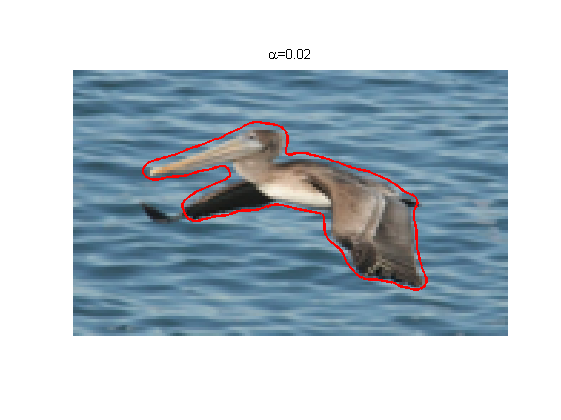
\includegraphics[width=45mm]{img/ex2/alpha/0_02.png}}
\subfigure[$ \alpha = 0.05 $]{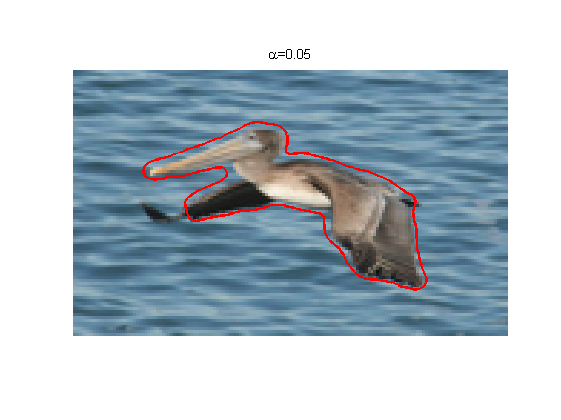
\includegraphics[width=45mm]{img/ex2/alpha/0_05.png}}
\subfigure[$ \alpha = 0.1 $]{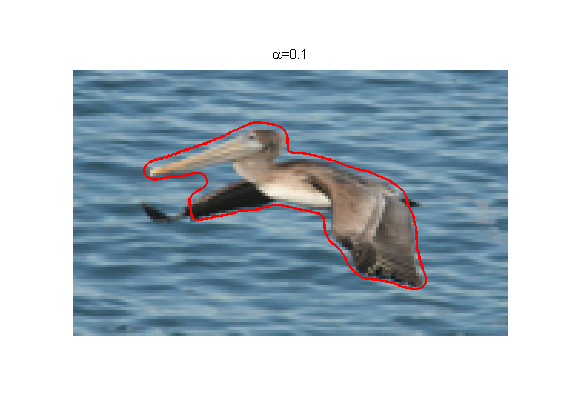
\includegraphics[width=45mm]{img/ex2/alpha/0_1.png}}

\subfigure[$ \alpha = 0.15 $]{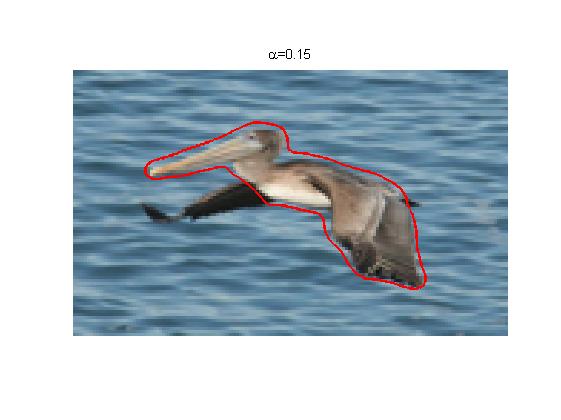
\includegraphics[width=45mm]{img/ex2/alpha/0_15.png}}
\subfigure[$ \alpha = 0.2 $]{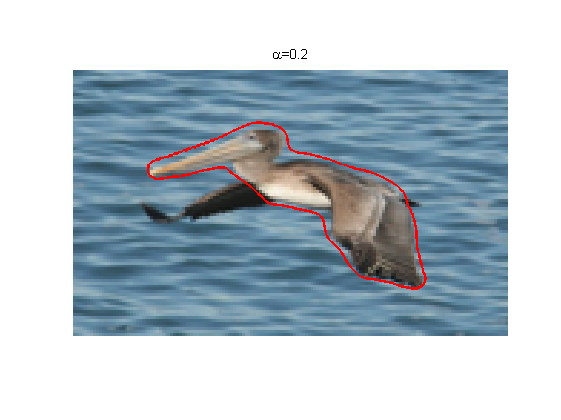
\includegraphics[width=45mm]{img/ex2/alpha/0_2.png}}
\caption{Bird: tweaking the value of $ \alpha $}
\label{fig:ex2-alpha-tweak}
\end{figure}

In figure \ref{fig:ex2-alpha-tweak} we can observe the effect of varying the $\alpha$ parameter.
We can see that at some point between $\alpha=0.1$ and $\alpha=0.15$ the right wing is left
outside of the segmented region. Therefore we consider the parameter $\alpha$ decisive for
the correct segmentation of the image, and we ascertain that its critical value is somewhat
higher than 0.1. This is, of course, starting from the default parameters. Due to the tight
relationship between the parameters the critical value can be altered when we modify the other
parameters.

\subsubsection{Beta}

\begin{figure}[!hbt]
\centering
\subfigure[$ \beta = 0 $]{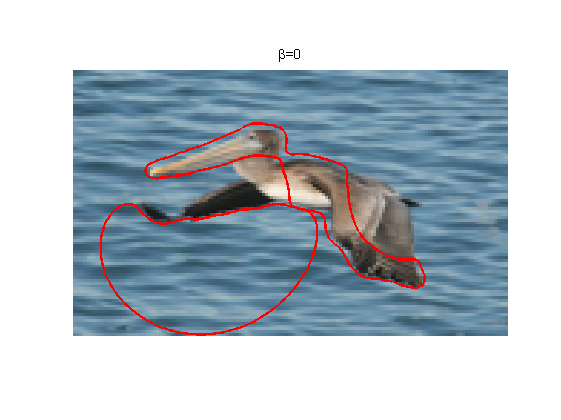
\includegraphics[width=45mm]{img/ex2/beta/0.png}}
\subfigure[$ \beta = 0.03 $]{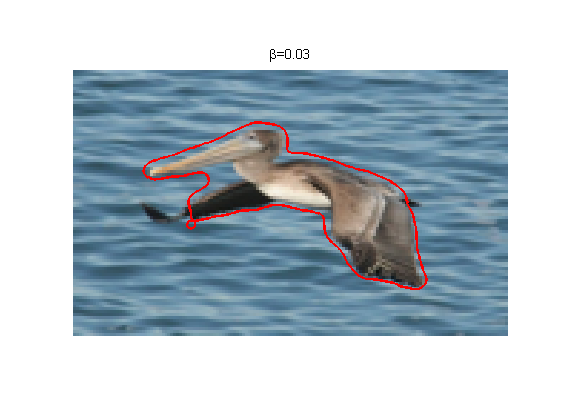
\includegraphics[width=45mm]{img/ex2/beta/0_03.png}}
\subfigure[$ \beta = 0.1 $]{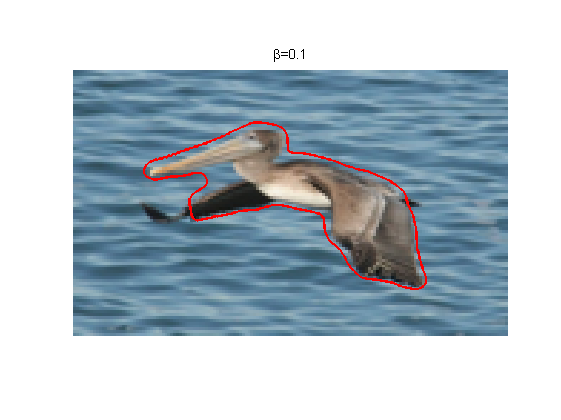
\includegraphics[width=45mm]{img/ex2/beta/0_1.png}}

\subfigure[$ \beta = 0.4 $]{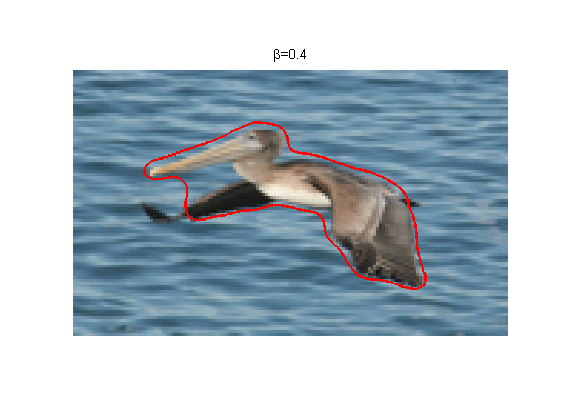
\includegraphics[width=45mm]{img/ex2/beta/0_4.png}}
\caption{Bird: tweaking the value of $ \beta $}
\label{fig:ex2-beta-tweak}
\end{figure}

In figure \ref{fig:ex2-beta-tweak} we can see that $ \beta $ is a very important parameter since
it can make the segmentation fail catastrophically. It seems that when we start from the default
values, the critical value is around 0.03. At this point the shape begins to twist on itself. High
values of $\beta$ can also yield a bad quality segmentation, producing a big gap between the edges of
the bird and the snake.

\subsubsection{Kappa}

\begin{figure}[!hbt]
\centering
\subfigure[$ \kappa' = 0.25 $]{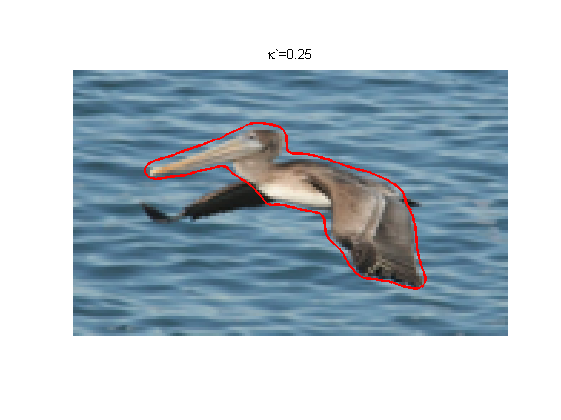
\includegraphics[width=45mm]{img/ex2/kappa/0_25.png}}
\subfigure[$ \kappa' = 0.3 $]{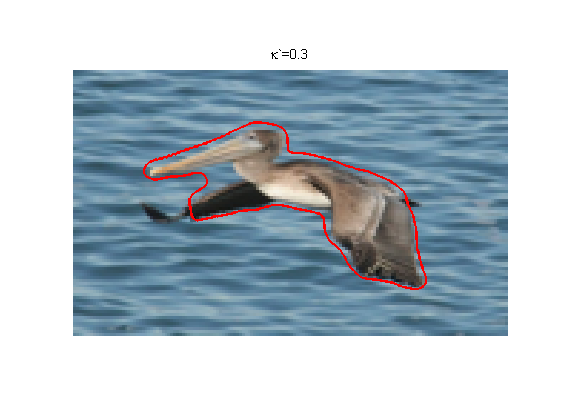
\includegraphics[width=45mm]{img/ex2/kappa/0_3.png}}
\subfigure[$ \kappa' = 0.4 $]{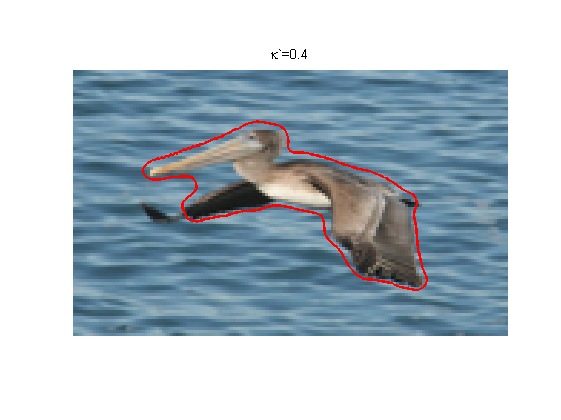
\includegraphics[width=45mm]{img/ex2/kappa/0_4.png}}

\subfigure[$ \kappa' = 1 $]{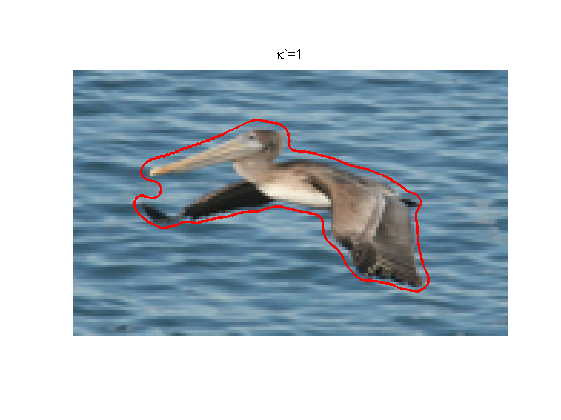
\includegraphics[width=45mm]{img/ex2/kappa/1.png}}
\caption{Bird: tweaking the value of $ \kappa' $}
\label{fig:ex2-kappa-tweak}
\end{figure}

As seen in figure \ref{fig:ex2-kappa-tweak}, tweaking the value of $\kappa'$ is one
of the possible strategies if we want the snake to fit around the right wing. The
parameter is very critical. Setting it lower than 0.2 lets the algorithm very prone
to crash (the snake shrinks to a singularity). On the other
hand, very low values can produce that the right wing is completely missed. We need
to set the value of $\kappa'$ higher if we want to correctly segment the wing. However
this requires to tweak the other parameters as well, since increasing the $ \kappa $ also
increases the gap between the snake and the bird.

\subsubsection{Lambda}

\begin{figure}[!hbt]
\centering
\subfigure[$ \lambda = -0.02 $]{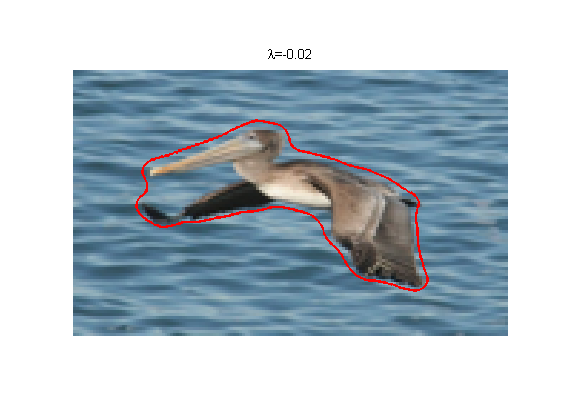
\includegraphics[width=45mm]{img/ex2/lambda/_0_02.png}}
\subfigure[$ \lambda = -0.04 $]{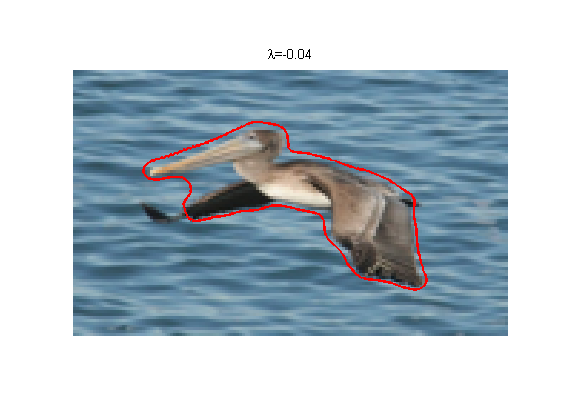
\includegraphics[width=45mm]{img/ex2/lambda/_0_04.png}}
\subfigure[$ \lambda = -0.05 $]{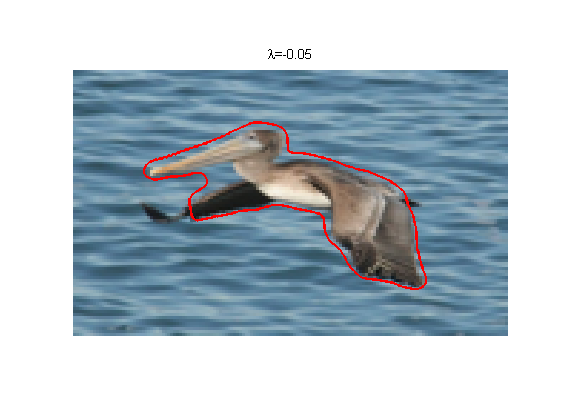
\includegraphics[width=45mm]{img/ex2/lambda/_0_05.png}}

\subfigure[$ \lambda = -0.055 $]{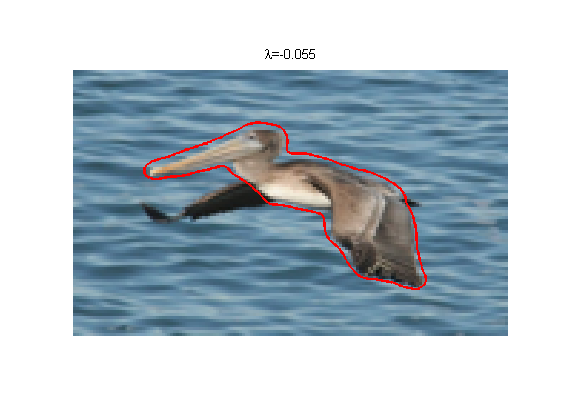
\includegraphics[width=45mm]{img/ex2/lambda/_0_055.png}}
\subfigure[$ \lambda = -0.06 $]{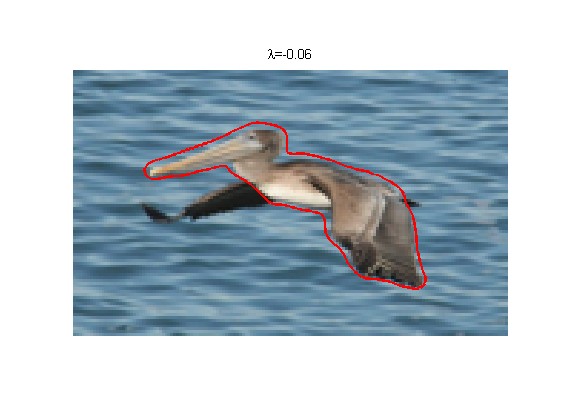
\includegraphics[width=45mm]{img/ex2/lambda/_0_06.png}}
\caption{Bird: tweaking the value of $ \lambda $}
\label{fig:ex2-lambda-tweak}
\end{figure}

In figure \ref{fig:ex2-lambda-tweak} we can appreciate the influence of $\lambda$. We can see
that its effect is very similar to that of $\kappa$, but inversed (which makes sense attending to
the meaning of those parameters). A high value (in absolute module) like -0.055 can make the
algorithm miss the wing completely while a low value makes the snake fit to the wing at the cost
of increasing the gap. Should this parameter be altered, we would need to modify one or more
of the other ones.

\subsubsection{Maxsteps}

\begin{figure}[!hbt]
\centering
\subfigure[$ \mathrm{maxsteps} = 0.02 $]{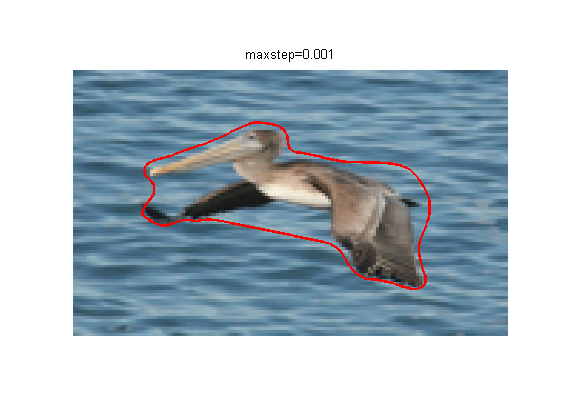
\includegraphics[width=45mm]{img/ex2/maxstep/0_001.png}}
\subfigure[$ \mathrm{maxsteps} = 0.01 $]{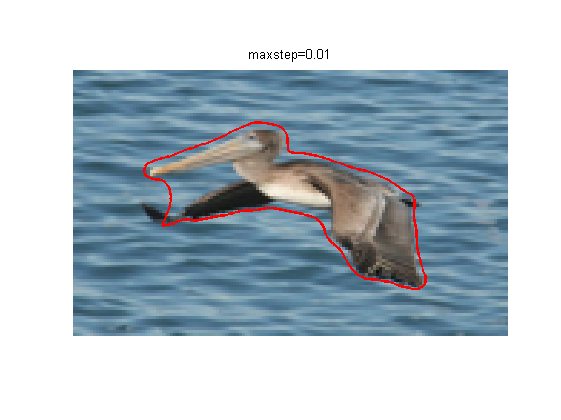
\includegraphics[width=45mm]{img/ex2/maxstep/0_01.png}}
\subfigure[$ \mathrm{maxsteps} = 0.4 $]{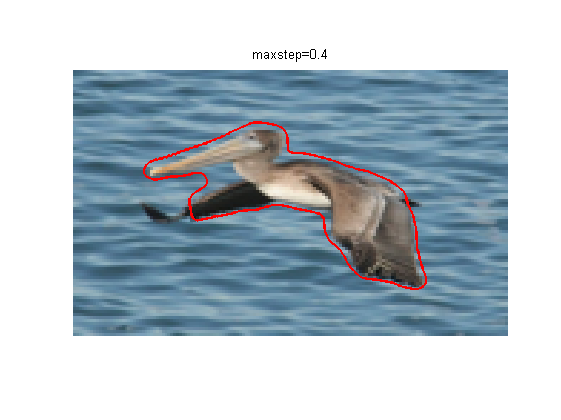
\includegraphics[width=45mm]{img/ex2/maxstep/0_4.png}}

\subfigure[$ \mathrm{maxsteps} = 1 $]{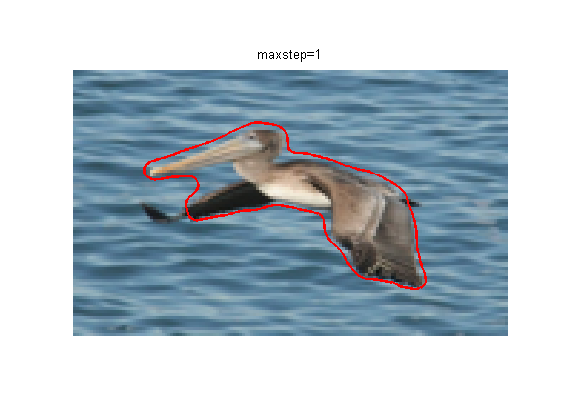
\includegraphics[width=45mm]{img/ex2/maxstep/1.png}}
\caption{Bird: tweaking the value of maxsteps}
\label{fig:ex2-maxsteps-tweak}
\end{figure}

Figure \ref{fig:ex2-maxsteps-tweak} shows that the influence of maxsteps is not too  high unless
it is low enough. A value higher than 0.4 does not seem to have a big impact, while values lower
than 0.01 seems to harm the quality of the result. Later we will see that this parameter can prevent the snake from crossing over, and therefore can be useful in the presence of noise.

\subsubsection{``Optimum values''}

As it can be seen in figure \ref{fig:ex2-alpha-tweak} for
$ \alpha = 0.1 $ (or for any of the plots in which the tweaked variable takes the default value), the right wing is not correctly segmented when the image
is scaled at 0.25 of its original dimensions. After taking note of the effect of each parameter
and performing some manual tweaking we have come to a set of values that effectively segmentates the bird when the image is scaled to 0.25, 0.5 and 1.0 of its original dimensions. These values are as follows:

\[ (\alpha , \beta , \kappa' , \lambda , \mathrm{maxstep} ) = (0.1, 0.03, 0.8, -0.08, 0.4) \]

While these values are not optimum in a mathematical sense, empirically they have rendered good results. The segmented image is shown in figure \ref{fig:bird-segmentated}.

\begin{figure}[!hbt]
\centering
\subfigure[$ \mathrm{maxsteps} = 0.02 $]{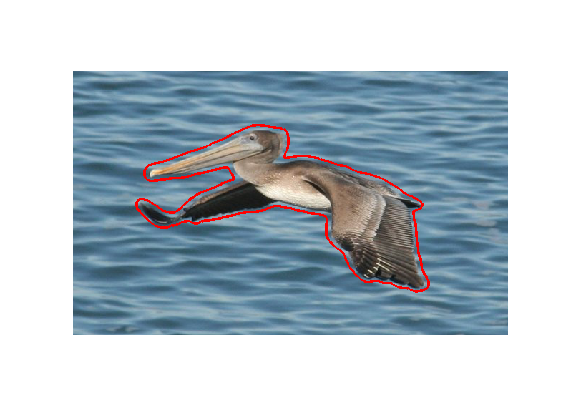
\includegraphics[width=45mm]{img/ex2/bird_segmentated_1x.png}}
\subfigure[$ \mathrm{maxsteps} = 0.01 $]{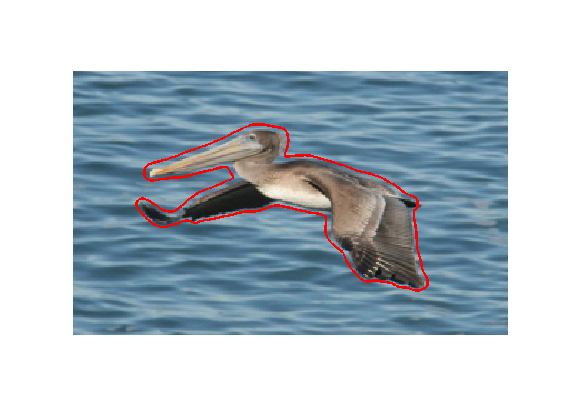
\includegraphics[width=45mm]{img/ex2/bird_segmentated_half.png}}
\subfigure[$ \mathrm{maxsteps} = 0.4 $]{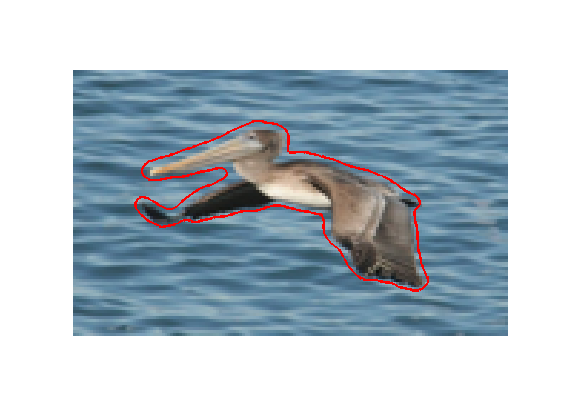
\includegraphics[width=45mm]{img/ex2/bird_segmentated_quarter.png}}
\caption{Bird: segmentation with ``optimum'' parameters at different scales}
\label{fig:bird-segmentated}
\end{figure}

\subsection{External force}

Much like in the previous case the external forces are a weighted combination of the force fields and the balloon force, being $\kappa$ and $\lambda$ the weights, respectively.

Also like before, the force field is obtained as the gradient of the smoothed grayscale image. This more or less the same concept than applying a Gaussian derivative filter to an image to extract its edges. The normalized force fields are shown in figure \ref{fig:bird-ff}.

\begin{figure}[!hbt]
\centering   
\subfigure[x dimension]{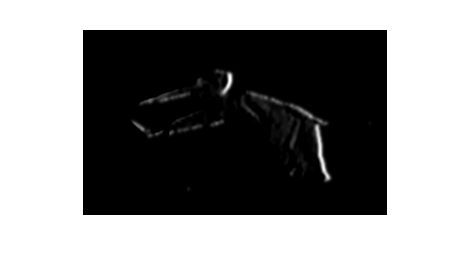
\includegraphics[width=60mm]{img/ex2/bird_efx.png}}
\subfigure[y dimension]{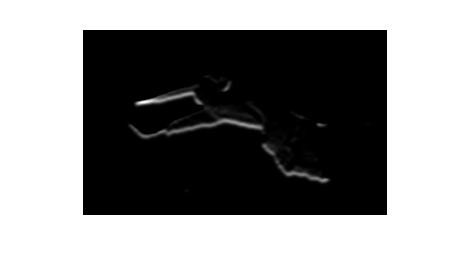
\includegraphics[width=60mm]{img/ex2/bird_efy.png}}
\caption{Force field of bird segmentation}
\label{fig:bird-ff}
\end{figure}

\subsection{Influence of noise on the segmentation}

We analyze mainly two kinds of noise: Additive White Gaussian noise and salt\&pepper noise.

\subsubsection{Additive White Gaussian Noise (AWGN) }

We have observed that the algorithm is very vulnerable to this kind of noise. We start by adding very
small amount of noise, and then we slowly start increasing it. We start with our ``optimum'' values. The results are shown in figure \ref{fig:awgn}. It can be observed that the algorithm starts giving poor results when the variance of the noise is 0.000125.

\begin{figure}[!hbt]
\centering   
\subfigure[WGN with mean 0 and variance 0.000001]{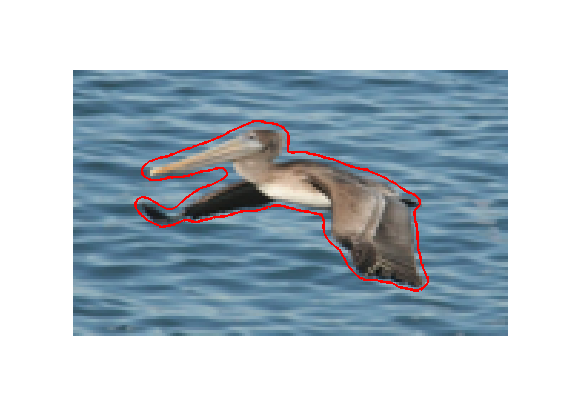
\includegraphics[width=45mm]{img/ex2/awgn/0_000001.png}}
\subfigure[WGN with mean 0 and variance 0.000005]{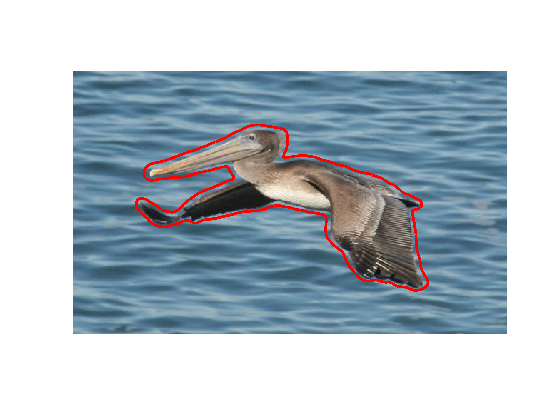
\includegraphics[width=45mm]{img/ex2/awgn/0_000005.png}}
\subfigure[WGN with mean 0 and variance 0.000025]{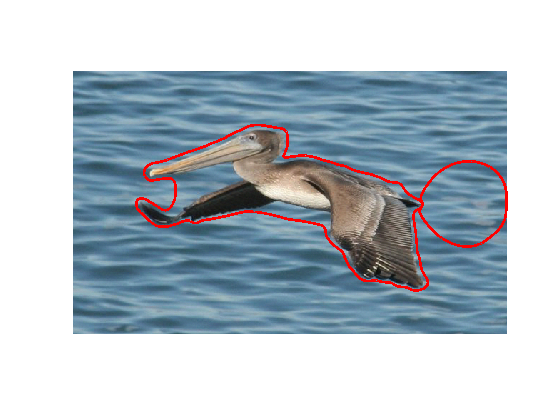
\includegraphics[width=45mm]{img/ex2/awgn/0_000025.png}}

\subfigure[WGN with mean 0 and variance 0.000125]{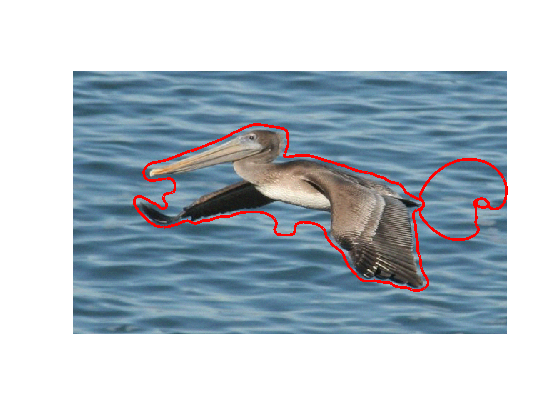
\includegraphics[width=45mm]{img/ex2/awgn/0_000125.png}}
\subfigure[WGN with mean 0 and variance 0.000625]{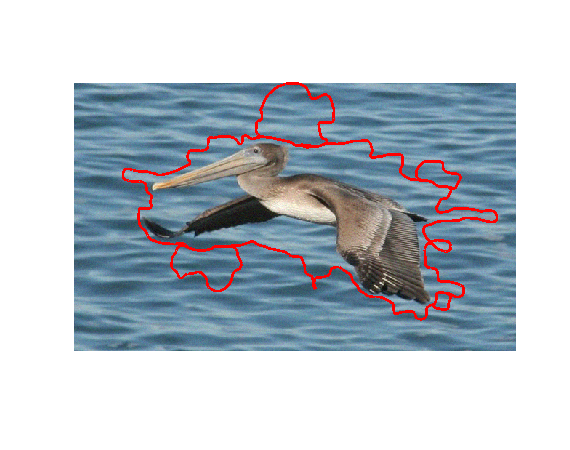
\includegraphics[width=45mm]{img/ex2/awgn/0_000625.png}}
\caption{Additive White Gaussian Noise}
\label{fig:awgn}
\end{figure}

These problems can be solved up to certain extend by tweaking the parameters. In particular, we reduce the maxstep parameter and increase the $\beta$ parameter to avoid twists. We also reduce $\kappa$ to avoid that the snake gets stuck too early in the algorithm. The results (shown in figure  \ref{fig:awgn-countermeasures} are subobptimal, but better than before).

\begin{figure}[!hbt]
\centering   
\subfigure[WGN with mean 0 and variance 0.000125]{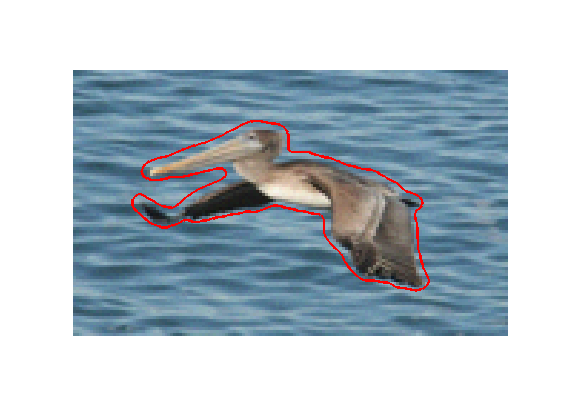
\includegraphics[width=45mm]{img/ex2/awgn/0_000125_fixed.png}}
\subfigure[WGN with mean 0 and variance 0.000625]{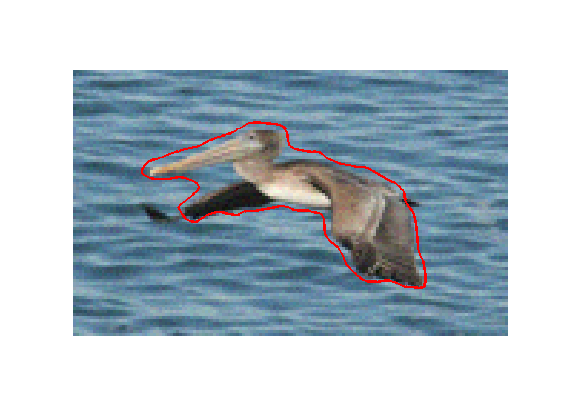
\includegraphics[width=45mm]{img/ex2/awgn/0_000625_fixed.png}}

\caption{Additive White Gaussian Noise: countermeasures}
\label{fig:awgn-countermeasures}
\end{figure}

\subsubsection{Salt and pepper}

In this case the situation is more grim than with AWGN. Even with very low densities of salt \& pepper noise the algorithm fails to converge to a solution consistently without the snake twisting over itself. The results are shown in figure \ref{fig:salt-pepper}

\begin{figure}[!hbt]
\centering   
\subfigure[Salt \& pepper with density 0.00001]{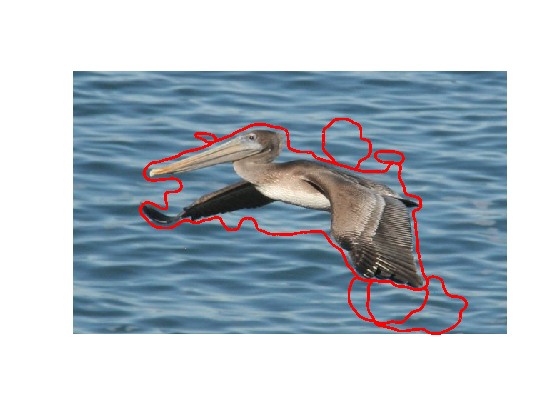
\includegraphics[width=45mm]{img/ex2/saltpepper/0_00001.png}}
\subfigure[Salt \& pepper with density 0.0001]{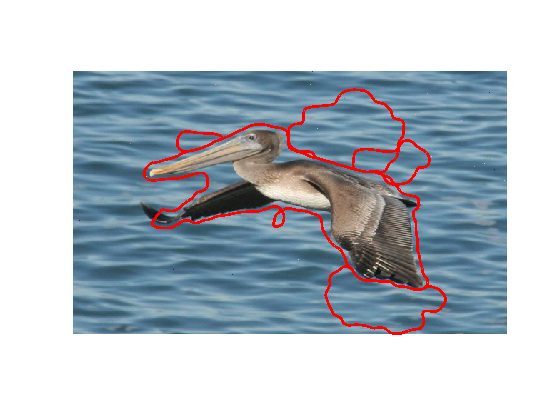
\includegraphics[width=45mm]{img/ex2/saltpepper/0_0001.png}}
\subfigure[Salt \& pepper with density 0.001]{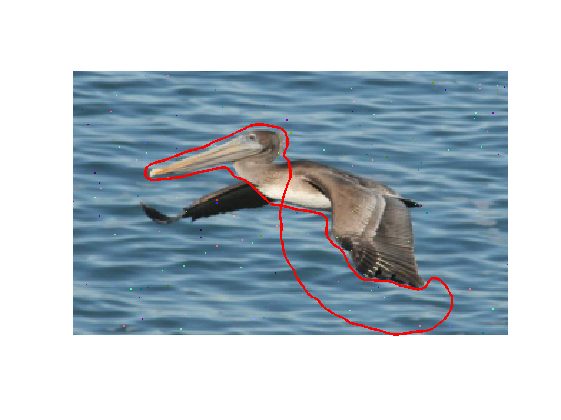
\includegraphics[width=45mm]{img/ex2/saltpepper/0_001.png}}

\caption{Salt \& pepper noise}
\label{fig:salt-pepper}
\end{figure}

While tuning the parameters could lead to segment the image correctly in some circumstances, the results were not consistent enough to be of any utility. When dealing with impulsive noise, like in our case, we would recommend applying a median filter first.
